\documentclass[conference]{IEEEtran}

\usepackage{cite}
\usepackage{amsmath,amssymb,amsfonts}
\usepackage{graphicx}
\usepackage{textcomp}
\usepackage{booktabs}
\usepackage{tabularx}
\usepackage{multirow}
\usepackage{array}
\usepackage{url}
\usepackage{tikz}
\usetikzlibrary{arrows.meta,positioning,fit,calc}

\hyphenation{Web-Sen-ti-nel Fast-API Post-gre-SQL}

\begin{document}

\title{WebSentinel: An Explainable Website Security Assessment and Phishing Detection System}

% =====================================================================
% AUTHOR BLOCK --- OPTION A (default): all project members
% Comment this block and uncomment Option B to list only the
% research-paper preparation team.
% =====================================================================
\author{
\IEEEauthorblockN{Seethina Jaya Dileep\IEEEauthorrefmark{1},
Ganesh Maheshwaram\IEEEauthorrefmark{1},
N V Sai Gokul\IEEEauthorrefmark{1},
Somineni Venumadhava\IEEEauthorrefmark{1},
Ruthwik Kakumani\IEEEauthorrefmark{1}, and
Ganta Sai Mani Chand\IEEEauthorrefmark{1}}
\IEEEauthorblockA{\IEEEauthorrefmark{1}Department: INSERT DEPARTMENT, University: INSERT UNIVERSITY\\
City: INSERT CITY, Country: INSERT COUNTRY\\
Email: INSERT EMAIL (Dileep public contact: jayadileepseethina@gmail.com)}
}

% =====================================================================
% AUTHOR BLOCK --- OPTION B: research-paper team only
% (Ruthwik Kakumani, Somineni Venumadhava, Seethina Jaya Dileep)
% =====================================================================
% \author{
% \IEEEauthorblockN{Ruthwik Kakumani\IEEEauthorrefmark{1},
% Somineni Venumadhava\IEEEauthorrefmark{1}, and
% Seethina Jaya Dileep\IEEEauthorrefmark{1}}
% \IEEEauthorblockA{\IEEEauthorrefmark{1}Department: INSERT DEPARTMENT, University: INSERT UNIVERSITY\\
% City: INSERT CITY, Country: INSERT COUNTRY\\
% Email: INSERT EMAIL}
% }

\maketitle

\begin{abstract}
Users routinely receive website addresses through electronic mail, messaging platforms, advertisements, QR codes, and social media. Non-technical users generally cannot determine whether a destination is legitimate, newly registered, misconfigured, or associated with phishing. Useful evidence---domain age, certificate status, DNS configuration, redirect behavior, hosting attributes, and reputation---exists in public sources, yet it is fragmented across independent services and is rarely presented as an accountable assessment. HTTPS alone does not establish trustworthiness, because phishing sites frequently obtain valid certificates. This paper presents WebSentinel, a website security assessment design that aggregates publicly observable indicators into a single explainable risk score in $[0,100]$ and a list of human-readable reasons. The proposed architecture combines safe URL validation, HTTP and TLS inspection, domain-registration analysis, and---in later stages---DNS, redirect, technology, reputation, and machine-learning components. A working prototype already implements origin-only URL intake, HTTPS and TLS checks, WHOIS-derived domain-age scoring, and a rule-based explanation list, delivered as a browser extension and a REST service. The paper specifies a weighted risk model, a planned phishing-classification pipeline with candidate learners, and scanner-side controls against server-side request forgery. No trained model metrics or large-scale scan statistics are reported, because those measurements were not present in the inspected implementation. The contribution is therefore a documented, ethically constrained assessment architecture and an implemented rule-based prototype, together with an evaluation plan that can be completed once datasets and tests are executed.
\end{abstract}

\begin{IEEEkeywords}
Phishing detection, website security, cybersecurity, machine learning, explainable artificial intelligence, URL analysis, threat intelligence, web security.
\end{IEEEkeywords}

\section{Introduction}
Phishing remains one of the most effective social-engineering attacks on the public web. Attackers impersonate banks, payment processors, cloud consoles, and social-network login pages in order to harvest credentials or payment data~\cite{dhamija2006why,apwg2024q4}. The Anti-Phishing Working Group continues to document large quarterly volumes of phishing activity, and the lifetime of many campaigns is short enough that purely reactive blacklists lag behind newly registered hosts~\cite{apwg2024q4,marchal2014phishstorm}. Browser security indicators help some users, but a substantial fraction of people do not inspect the address bar or certificate UI, and visual deception can still succeed~\cite{dhamija2006why}.

\subsection{Background}
Public information about a website is abundant. The URL itself encodes scheme, hostname, and path~\cite{rfc3986}. HTTP semantics describe status codes and redirects~\cite{rfc9110}. DNS records associate names with addresses and mail exchangers~\cite{rfc1035}. Registration data---historically WHOIS and increasingly RDAP---expose creation dates, registrars, and nameservers~\cite{rfc7480,rfc7483}. X.509 certificates describe issuer, validity interval, and subject binding~\cite{rfc5280,rfc8446}. Threat-intelligence services maintain reputation for known-bad hosts. Each of these channels has been used, separately, in prior anti-phishing research~\cite{zhang2007cantina,ma2009beyond,xiang2011cantinaplus,rao2019detection}. Ordinary users, however, cannot query and interpret these sources under time pressure.

\subsection{Problem Statement}
The operational problem is therefore not the absence of security signals. It is the combination of (i)~fragmented evidence, (ii)~a user population that cannot interpret raw WHOIS or certificate fields, and (iii)~phishing sites that imitate legitimate brands and often present a padlock icon. A URL received in SMS, email, or a QR code may be a look-alike domain, a newly registered host, an open redirect, or a page served over HTTPS from an otherwise suspicious infrastructure. Existing commercial toolbars and Safe Browsing-style classifiers are effective at scale~\cite{whittaker2010large} but typically return an opaque block-or-allow decision. Academic detectors that rely only on lexical URL features, only on page content, or only on search-engine queries each miss complementary evidence~\cite{sahingoz2019ml,hannousse2021benchmark}.

WebSentinel addresses this gap by aggregating several publicly observable indicators into one assessment and by explaining \emph{why} a site appears comparatively safe or comparatively risky. The system is intended as an advisory assistant. A low score is not a proof of safety; a high score is a request for caution.

\subsection{Research Motivation}
University-capstone and small-organization settings rarely operate a full security-operations pipeline. They still, however, click unknown links. A system that performs only passive or otherwise approved checks against public information---and that refuses to exploit, credential-harvest, or attack the target---is an appropriate response. The same URL-fetching capability can become a vulnerability if the scanner is induced to contact loopback, RFC~1918, or cloud-metadata addresses~\cite{rfc1918,rfc6890,owaspssrf}. Designing the scanner so that it cannot be turned into an internal probe is therefore part of the research problem, not an afterthought.

\subsection{Objectives}
The work pursues the following objectives.
\begin{enumerate}
  \item Aggregate important website-security information in a single system.
  \item Identify common phishing and suspicious-website indicators.
  \item Analyze HTTP, DNS, RDAP or domain-registration, IP, TLS, redirect, and technology signals, to the extent each collector is implemented.
  \item Generate an explainable risk score in $[0,100]$.
  \item Explain individual warnings in language suitable for non-technical users.
  \item Store previous scans and generate downloadable reports (\emph{planned}).
  \item Incorporate machine-learning phishing prediction and approved threat-intelligence sources (\emph{planned}).
  \item Support website monitoring and change detection (\emph{planned}).
  \item Maintain safe and ethical assessment practices, including SSRF-aware URL handling.
\end{enumerate}

\subsection{Main Contributions}
This paper makes four contributions.
\begin{itemize}
  \item A threat model and ethical scanning boundary for a user-facing website assessment service, including scanner-side SSRF as a first-class risk~\cite{owaspssrf,owasp2021top10}.
  \item A proposed multi-collector architecture that unifies protocol, registration, DNS, TLS, redirect, technology, reputation, and (later) learning-based signals under one risk engine.
  \item A documented prototype, inspected in source form, that already implements origin-only intake, HTTPS and TLS checks, WHOIS-derived age scoring, and natural-language reasons.
  \item An evaluation methodology and table templates for functional, security, performance, and machine-learning experiments, without fabricated numerical results.
\end{itemize}

The remainder of the paper is organized as follows. Section~\ref{sec:related} reviews related work. Section~\ref{sec:threat} states requirements and the threat model. Section~\ref{sec:arch} describes the proposed architecture and the implemented subset. Section~\ref{sec:method} presents the methodology. Section~\ref{sec:impl} discusses implementation choices. Sections~\ref{sec:setup}--\ref{sec:results} cover experimental design, testing, and the current absence of measured results. Sections~\ref{sec:privacy}--\ref{sec:future} address privacy, limitations, and future work. Section~\ref{sec:concl} concludes.

\section{Related Work}
\label{sec:related}
Phishing detection research has evolved from content heuristics and blacklists toward lexical learning, hybrid feature models, visual brand matching, and explainable decision support. This section reviews those lines and positions WebSentinel conceptually against them. Table~\ref{tab:comparison} summarizes the comparison.

\subsection{User Studies and the Limits of Browser Cues}
Dhamija \emph{et al.} showed that many users ignore certificate and address-bar cues and that visual spoofing remains effective even against comparatively sophisticated participants~\cite{dhamija2006why}. That finding motivates systems that translate technical evidence into short reasons rather than assuming that a padlock icon is sufficient.

\subsection{Content-Based and Search-Based Detectors}
CANTINA applied TF--IDF robust hyperlinks to decide whether page terms are consistent with a legitimate site, optionally combined with heuristics~\cite{zhang2007cantina}. CANTINA+ expanded the feature set with DOM, search-engine, and third-party attributes and added filters for near-duplicate phishing pages and login-form absence~\cite{xiang2011cantinaplus}. PhishStorm computed intra-URL relatedness from search-query data and produced a phishingness rating suitable for streaming deployment~\cite{marchal2014phishstorm}. These systems demonstrated that content and search context can catch pages that lexical rules miss, at the cost of search-API dependence and page-download overhead. WebSentinel's prototype does not fetch page HTML for classification; content and technology analysis remain planned.

\subsection{URL and Host Feature Learning}
Ma \emph{et al.} showed that lexical and host features can classify malicious URLs without downloading page bodies, and that online learning is well suited to drifting URL streams~\cite{ma2009beyond,ma2009identifying}. Subsequent work engineered richer URL tokenizations and NLP-style features. Sahingoz \emph{et al.} compared seven classifiers on a large URL corpus and reported strong Random Forest performance with language-independent NLP features~\cite{sahingoz2019ml}. CatchPhish inspected URL structure without relying on page content~\cite{rao2019catchphish}. Character-level convolutional networks learn sequential patterns directly from the URL string and avoid some hand-crafted features~\cite{aljofey2020cnn}. Hybrid models combine address-bar features with hyperlink or third-party attributes~\cite{rao2019detection,dasguptta2024hybrid}. Hannousse and Yahiouche argued for reproducible feature-rich benchmarks and released a balanced dataset with URL, content, and external-service features~\cite{hannousse2021benchmark,hannousse2021dataset}. Neural and rule-extraction models on structured phishing-website features were studied earlier by Mohammad \emph{et al.}~\cite{mohammad2014predicting}. PhishMon emphasized efficiently computable page features that are costly for attackers to emulate~\cite{niakanlahiji2018phishmon}.

These studies consistently find that accuracy alone is an incomplete metric: false negatives expose users to credential theft, while false positives erode trust. They also show that external features (registration age, DNS, reputation) are often highly discriminative but introduce latency and third-party failure modes~\cite{hannousse2021benchmark}. WebSentinel follows that hybrid philosophy while insisting that every fired indicator be explainable to a non-expert.

\subsection{Reputation, Blacklists, and Browser Protection}
Industry detectors such as the large-scale classifier described by Whittaker \emph{et al.} combine crawling, content features, and continually updated labels~\cite{whittaker2010large}. Blacklists are effective for known campaigns and weak against zero-hour hosts~\cite{marchal2014phishstorm,apwg2024q4}. WebSentinel treats approved reputation lookups as an optional planned signal, not as the sole decision source.

\subsection{Visual Similarity and Brand Impersonation}
VisualPhishNet learns trusted-site visual profiles with a triplet CNN~\cite{abdelnabi2020visualphishnet}. Phishpedia identifies brand logos and matches them to claimed identities, producing an explanation in the form of a target brand~\cite{lin2021phishpedia}. Those approaches are complementary to WebSentinel's current host-and-certificate focus and are listed as future work rather than implemented modules.

\subsection{Explainable Machine Learning in Security}
LIME explains individual classifier predictions by local linear surrogates~\cite{ribeiro2016lime}. SHAP assigns consistent additive feature attributions grounded in Shapley values~\cite{lundberg2017shap}. Phishing tools that emit only a probability leave users unable to judge whether HTTPS, domain age, or a lexical oddity dominated the decision. The proposed second-semester design therefore treats SHAP (or an equivalent attribution method) as the explanation layer for any learned model. The current prototype explains decisions with deterministic rule texts, which are already a form of inherent interpretability.

\subsection{Standards Relevant to Collectors and Scanner Safety}
URI syntax~\cite{rfc3986}, HTTP semantics~\cite{rfc9110}, DNS~\cite{rfc1035}, TLS~1.3~\cite{rfc8446}, and the Internet X.509 PKI profile~\cite{rfc5280} constrain what a passive scanner may observe. RDAP specifies HTTP/JSON access to registration data as a successor to WHOIS~\cite{rfc7480,rfc7483}. Private and special-purpose address registries enumerate destinations that a URL scanner must not fetch~\cite{rfc1918,rfc6890}. OWASP documents SSRF as a systemic web risk and publishes a prevention cheat sheet~\cite{owasp2021top10,owaspssrf}.

\subsection{Positioning}
Relative to prior work, WebSentinel is not a new deep classifier and does not claim visual brand matching. Its intended niche is a unified, user-explainable assessment that (i)~already ships a conservative rule engine on HTTPS, certificates, and domain age, and (ii)~is specified to grow toward DNS, redirects, technologies, reputation, and a documented ML pipeline without converting the scanner into an attack tool. Table~\ref{tab:comparison} makes that distinction explicit by separating the inspected prototype from the proposed system.

\begin{table*}[!t]
\centering
\caption{Conceptual comparison of WebSentinel with representative prior approaches.}
\label{tab:comparison}
\renewcommand{\arraystretch}{1.12}
\begin{tabular}{>{\raggedright\arraybackslash}p{2.7cm}cccccccc}
\toprule
Approach & URL & DNS & SSL & Age & TI & ML & XAI & Score \\
\midrule
CANTINA~\cite{zhang2007cantina} & P & -- & -- & P & P & -- & L & -- \\
CANTINA+~\cite{xiang2011cantinaplus} & Y & P & -- & P & Y & Y & L & -- \\
PhishStorm~\cite{marchal2014phishstorm} & Y & -- & -- & -- & P & Y & P & P \\
URL ML~\cite{sahingoz2019ml,rao2019catchphish} & Y & -- & -- & -- & -- & Y & L & -- \\
Hybrid ML~\cite{rao2019detection,dasguptta2024hybrid} & Y & P & P & P & P & Y & L & -- \\
Safe Browsing-style~\cite{whittaker2010large} & Y & -- & -- & -- & Y & Y & -- & -- \\
Visual~\cite{lin2021phishpedia,abdelnabi2020visualphishnet} & -- & -- & -- & -- & -- & Y & P & -- \\
Prototype (this work) & P & -- & Y & Y & -- & -- & Y & Y \\
Proposed system & Y & Y & Y & Y & Y & Y & Y & Y \\
\bottomrule
\end{tabular}
\vspace{2pt}
{\footnotesize Y: primary; P: partial; L: limited; TI: threat intelligence; Age: domain age; XAI: explanation; Score: unified 0--100 risk score. Prototype versus proposed rows reflect inspected code, not aspiration presented as fact.}
\end{table*}

\section{System Requirements and Threat Model}
\label{sec:threat}

\subsection{Intended Users}
The primary user is a non-expert who received a link and wants a short, reasoned caution level before entering credentials. Secondary users are student analysts and small-team operators who need a stored history of assessments (\emph{planned}) and a downloadable report (\emph{planned}). The system is not a penetration-testing platform and is not authorized to assess systems that the user does not have a legitimate reason to inspect as a public client.

\subsection{Assets}
Protected assets are (i)~the user's credentials and session tokens, which must never be requested or stored; (ii)~the confidentiality of the submitted URL, of which the prototype already minimizes path and query; and (iii)~the scanner host itself, including any cloud-metadata credentials reachable via SSRF.

\subsection{Attacker Model}
The external attacker crafts URLs and websites intended to impersonate trusted brands. The attacker may register a young domain, obtain a valid publicly trusted certificate, use many subdomains, employ redirects, copy HTML and logos, and rotate hosting. The attacker may also try to cause false negatives by presenting HTTPS and a plausible brand, or false positives against WebSentinel by mimicking aged, well-configured infrastructure (a residual risk). A second adversary is a user of the scanner---or a page that tricks a user into scanning a URL---who attempts to make the backend fetch internal resources. That adversary is modeled as an SSRF attacker~\cite{owaspssrf}.

\subsection{Phishing and Malicious-URL Threat}
Phishing pages seek credentials, session cookies, cryptocurrency, or malware delivery. They are often short-lived~\cite{hannousse2021benchmark,apwg2024q4}. Malicious URLs more broadly include drive-by exploit hosts and spam landing pages~\cite{ma2009beyond}. WebSentinel's current rules target \emph{suspiciousness indicators} correlated with phishing and poor operational hygiene; they do not prove criminal intent.

\subsection{Ethical Scanning Boundaries}
The system must not steal credentials, attempt exploitation, perform destructive testing, bypass authentication, or conduct unauthorized attacks. Collectors are restricted to information a normal web client or public directory service can observe: scheme, certificate on port 443, and registration records. Future HTML fetches, if enabled, must remain unauthenticated GET requests with strict timeouts and size limits. Approved threat-intelligence APIs may be queried only under their terms of use.

\subsection{System Limitations as Requirements}
The service cannot see authenticated application state, cannot execute a full browser DOM without a planned headless client, and cannot guarantee completeness of WHOIS or RDAP fields. Those limits are accepted: the output is advisory.

\subsection{SSRF Threat Against the Scanner}
If a user can supply \texttt{http://127.0.0.1/}, \texttt{http://169.254.169.254/}, an RFC~1918 literal, a DNS name that resolves to such an address, or a redirect that later targets one, the scanner becomes an internal HTTP proxy~\cite{rfc1918,rfc6890,owaspssrf}. Cloud instance-metadata endpoints are a documented high-value target. The proposed control set is specified in Section~\ref{sec:ssrf}. The inspected prototype validates scheme and strips path, but it does not yet enforce private-address denial after DNS resolution. That gap is treated as an implementation debt, not as a completed control.

\section{Proposed System Architecture}
\label{sec:arch}
Fig.~\ref{fig:arch} depicts the proposed architecture. The current prototype occupies a strict subset of that figure: a Manifest~V3 Chrome popup, an Express.js API, and three collectors (protocol, TLS, WHOIS).

\begin{figure}[!t]
\centering
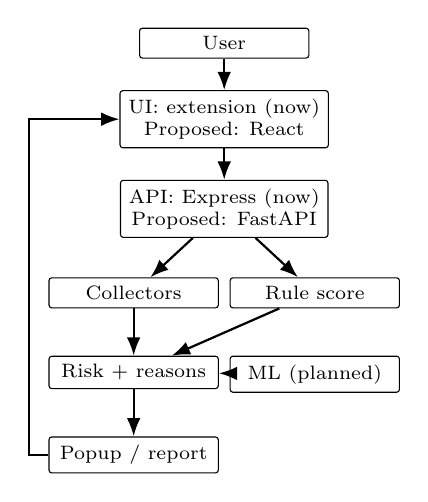
\begin{tikzpicture}[
  font=\scriptsize,
  box/.style={draw, rounded corners=1pt, align=center, inner sep=3pt, minimum width=2.15cm},
  arr/.style={-{Latex}, thick}
]
\node[box] (user) {User};
\node[box, below=4mm of user] (ui) {UI: extension (now)\\Proposed: React};
\node[box, below=4mm of ui] (api) {API: Express (now)\\Proposed: FastAPI};
\node[box, below=5mm of api, xshift=-1.15cm] (col) {Collectors};
\node[box, below=5mm of api, xshift=1.15cm] (rule) {Rule score};
\node[box, below=6mm of col] (risk) {Risk + reasons};
\node[box, below=6mm of rule] (ml) {ML (planned)};
\node[box, below=6mm of risk] (out) {Popup / report};
\draw[arr] (user) -- (ui);
\draw[arr] (ui) -- (api);
\draw[arr] (api) -- (col);
\draw[arr] (api) -- (rule);
\draw[arr] (col) -- (risk);
\draw[arr] (rule) -- (risk);
\draw[arr] (ml) -- (risk);
\draw[arr] (risk) -- (out);
\draw[arr] (out.west) -- ++(-0.25,0) |- (ui.west);
\end{tikzpicture}
\caption{Proposed architecture of the WebSentinel security assessment system. The prototype implements the UI, API, collector, and rule-score path.}
\label{fig:arch}
\end{figure}

\subsection{Frontend}
The \emph{proposed} user interface is a React, TypeScript, and Tailwind CSS dashboard with URL entry, scan history, and report download. The \emph{implemented} interface is a Chrome extension popup (\texttt{frontend/index.html}, \texttt{frontend/app.js}) that reads the active tab, rejects non-HTTP(S) schemes locally, posts only the origin, and renders a verdict (\texttt{Safe}, \texttt{Suspicious}, \texttt{High risk}), a numeric score, and a ``Why'' list. The extension requests \texttt{activeTab} and a single API host permission.

\subsection{Backend}
The proposed backend is an asynchronous FastAPI service that orchestrates collectors and the risk engine. The implemented backend is Express.js~5 (\texttt{backend/server.js}) exposing \texttt{GET /health} and \texttt{POST /check}, with an 8~kB JSON body limit and CORS enabled. Local listening is bound to \texttt{127.0.0.1} unless deployed on Vercel.

\subsection{Data-Collection Modules}
Proposed collectors cover HTTP responses, DNS, RDAP, TLS, redirects, IP/hosting/geolocation, HTML technology fingerprints, and optional reputation APIs. Implemented collectors are: scheme inspection (\texttt{testhttp.js}); TLS inspection via \texttt{ssl-checker} (\texttt{testssl.js}); and domain-registration scraping of a public WHOIS HTML endpoint (\texttt{testdata.js}). A file \texttt{rdap.js} exists but is empty; RDAP is therefore planned, not implemented.

\subsection{Database}
The proposed schema includes users, scans, websites, domain records, DNS records, TLS records, redirects, technologies, risk findings, ML predictions, reports, and monitoring configurations. The inspected prototype persists nothing: each check is stateless. No PostgreSQL models were found.

\subsection{Background Processing}
Celery or RQ with Redis is specified for long scans and monitoring. The prototype performs collectors inline with \texttt{Promise.allSettled} and an 8~s per-collector timeout.

\subsection{Machine-Learning Module}
A scikit-learn classifier with optional SHAP explanations is planned for semester two. No model artifact, training notebook, or feature-store code was found.

\subsection{Risk Engine and Report Generator}
The implemented engine is the additive penalty function in \texttt{testingmain.js}. Downloadable reports and a React report view are planned.

\subsection{External Threat Intelligence}
Approved breach or reputation APIs are planned. None are called in the inspected code.

\section{Methodology}
\label{sec:method}

\subsection{URL Validation}
\label{sec:urlval}
Let $u$ be the raw input. The prototype parses $u$ with the WHATWG URL parser, optionally prefixing \texttt{https://}. A request is rejected if the scheme is not \texttt{http} or \texttt{https}, or if it matches an unsupported family
\[
\{\texttt{chrome},\texttt{edge},\texttt{about},\texttt{devtools},\texttt{file},\texttt{data},\texttt{blob},\ldots\}.
\]
The API then discards path, query, and fragment and retains only
\[
\mathrm{origin}(u)=\mathrm{scheme}(u)\mathbin{||}\texttt{://}\mathbin{||}\mathrm{host}(u).
\]
This is a privacy control as well as a validation step: secrets encoded in query strings never leave the browser. Planned validation additionally resolves $\mathrm{host}(u)$ and refuses private, loopback, link-local, and metadata addresses (Section~\ref{sec:ssrf}).

\subsection{HTTP Analysis}
The prototype does not issue a full HTTP GET to the target for header or body analysis. It only tests whether the scheme is HTTPS~\cite{rfc9110}. Planned HTTP analysis will record status code, selected security headers, and title or description from a size-limited GET, still without authentication.

\subsection{DNS Analysis}
Planned. A resolver (for example, \texttt{dnspython}) would collect A, AAAA, MX, NS, and TXT records~\cite{rfc1035}. The prototype currently surfaces nameservers only when the WHOIS scrape includes them; it does not perform independent DNS queries.

\subsection{Domain and RDAP Analysis}
RDAP is the standards-based successor to WHOIS~\cite{rfc7480,rfc7483}. The prototype instead HTTP-GETs a third-party WHOIS presentation page and parses embedded JSON. Extracted fields include registrar, creation, update, and expiration dates, nameservers, and a DNSSEC string. Domain age is computed from the creation timestamp as a $(y,m,d)$ triple. This collector is a functional stand-in for RDAP and inherits HTML-structure brittleness; replacing it with RDAP is planned.

\subsection{SSL/TLS Analysis}
The prototype connects to port 443 with an 8~s timeout and records validity, validity interval, days remaining, and issuer~\cite{rfc5280,rfc8446}. An exception is treated as an invalid certificate. Planned work includes chain validation details and protocol-version reporting. HTTPS remains insufficient as a trust signal~\cite{dhamija2006why,apwg2024q4}.

\subsection{Redirect Analysis}
Planned. A bounded client should follow at most $N$ redirects, re-validate each hop against the SSRF policy, and flag cross-registrable-domain hops and excessive chain length.

\subsection{Technology Detection}
Planned. Header and HTML signatures (server, framework, CMS, libraries) would be collected with a size-capped parser. The prototype does not fetch HTML from the assessed site.

\subsection{Reputation Analysis}
Planned, and only through approved APIs. A positive hit is an indicator, not an automatic legal determination.

\subsection{Feature Extraction}
Let $\mathbf{x}$ be the feature vector. The prototype uses a small discrete set: HTTPS flag, certificate validity, days-to-expiry, domain-age bucket, WHOIS-update recency, and a DNSSEC string. The proposed vector additionally includes URL length, dot and subdomain counts, digit and special-character counts, IP-literal host, redirect count, lexical keywords, login-form cues, and reputation. Features should be computed from already-collected artifacts to avoid extra network risk.

\subsection{Rule-Based Risk Scoring}
\label{sec:score}
Two scoring presentations are distinguished.

\paragraph{Implemented prototype.}
Let $S$ be an integer initialized to $0$. Penalties observed in \texttt{testingmain.js} are
\begin{align}
S &\mathrel{+}= 20 && \text{if scheme is not HTTPS,} \nonumber\\
S &\mathrel{+}= 20 && \text{if the certificate is missing or invalid,} \nonumber\\
S &\mathrel{+}= 3 && \text{if } 0 \le d_{\mathrm{exp}} < 7, \nonumber\\
S &\mathrel{+}= a(y,m,d) && \text{age bucket,} \nonumber\\
S &\mathrel{+}= u(\Delta) && \text{WHOIS update recency,} \nonumber\\
S &\mathrel{-}= 3 && \text{if HTTPS and DNSSEC is signed.} \nonumber
\end{align}
The age function $a$ is mutually exclusive:
\[
a=
\begin{cases}
35, & y=m=0,\ d<7,\\
25, & y=0,\ m<1,\\
15, & y=0,\ m<6,\\
8, & y<1,\\
0, & \text{otherwise.}
\end{cases}
\]
Update recency $u(\Delta)$ is $10$ if $\Delta<7$ days, $6$ if $\Delta<30$, else $0$. The implementation then applies $S \leftarrow \max(S,0)$. Verdicts are
\[
\begin{cases}
\text{Safe,} & S<24,\\
\text{Suspicious,} & 24\le S<59,\\
\text{High risk,} & S\ge 59.
\end{cases}
\]
These thresholds are design choices in source code. They have not been experimentally calibrated on a labeled corpus.

\paragraph{Proposed normalized model.}
For a planned multi-signal engine, let $f_i\in[0,1]$ be a normalized risk contribution of indicator $i$ and $w_i\ge 0$ its weight. An optional learned probability $p\in[0,1]$ may be included with weight $\lambda$:
\begin{equation}
R_{\mathrm{raw}}=\sum_{i=1}^{n} w_i f_i + \lambda p,
\label{eq:raw}
\end{equation}
\begin{equation}
R = \mathrm{clip}_{[0,100]}\!\left(100\cdot\frac{R_{\mathrm{raw}}}{\sum_i w_i + \lambda}\right).
\label{eq:norm}
\end{equation}
A five-level interpretation may later be used,
\[
\begin{array}{ll}
{[}0,20{]} & \text{Very low risk,}\\
{[}21,40{]} & \text{Low risk,}\\
{[}41,60{]} & \text{Moderate risk,}\\
{[}61,80{]} & \text{High risk,}\\
{[}81,100{]} & \text{Very high risk,}
\end{array}
\]
but those bands are \emph{not} the bands running in the prototype and must not be presented as validated.

\subsection{Machine-Learning Classification}
\label{sec:ml}
No classifier is trained in the inspected repository. The planned pipeline is: obtain an approved dataset such as the Hannousse--Yahiouche benchmark~\cite{hannousse2021dataset,hannousse2021benchmark} or a similarly licensed PhishTank/OpenPhish plus legitimate crawl; clean and deduplicate; engineer $\mathbf{x}$; apply a stratified train/test split; fit candidate models (logistic regression, decision tree, random forest, gradient boosting) that have been effective on tabular phishing features~\cite{sahingoz2019ml,rao2019detection,hannousse2021benchmark,dasguptta2024hybrid}; and emit $p=\Pr(\mathrm{phish}\mid\mathbf{x})$. Class imbalance, if present, should be handled with class weights or resampling rather than ignored. Accuracy is insufficient because a trivial majority classifier can look strong on skewed data, and because a false negative (phishing labeled legitimate) has a higher user-safety cost than a false positive, which mainly costs convenience~\cite{xiang2011cantinaplus,sahingoz2019ml}. Precision, recall, F1-score, and ROC-AUC are therefore mandatory.

\subsection{Explainability}
Rule explanations in the prototype are the strings appended when a penalty fires (for example, ``Domain is extremely new \ldots''). For a future model $g(\mathbf{x})=p$, SHAP values $\phi_i$ satisfy
\begin{equation}
g(\mathbf{x})=\phi_0+\sum_i \phi_i,
\label{eq:shap}
\end{equation}
where $\phi_0$ is the baseline expectation~\cite{lundberg2017shap}. A user-facing explanation would list the largest positive $\phi_i$ (evidence for phishing) and negative $\phi_i$ (evidence against). A valid certificate should be allowed to appear as negative evidence without being described as proof of legitimacy. SHAP is planned; no SHAP values were computed in the inspected project.

\subsection{Safe Website Scanning and SSRF Controls}
\label{sec:ssrf}
The scanner is itself a confused deputy~\cite{owaspssrf}. The proposed control set, aligned with OWASP guidance, is:
\begin{enumerate}
  \item Allow only \texttt{http} and \texttt{https}.
  \item Normalize and reject credentials in the URL.
  \item Resolve DNS and apply an allow-or-deny decision on the \emph{resolved} address, not only on the literal hostname.
  \item Deny loopback, RFC~1918 private space, link-local, multicast, IPv6 unique-local, and well-known cloud-metadata addresses~\cite{rfc1918,rfc6890,owaspssrf}.
  \item Re-validate every redirect hop.
  \item Enforce connect and read timeouts, response-size limits, and a maximum redirect count.
  \item Rate-limit clients to reduce abuse as an open scanner.
\end{enumerate}
The prototype implements (1), path stripping, body-size limiting on the API, and collector timeouts. Items (3)--(7) are specified here as required engineering before any open deployment that fetches arbitrary URLs.

\section{Implementation}
\label{sec:impl}

\subsection{Implementation Status}
Table~\ref{tab:status} records what the inspected repository \texttt{seethinajayadileep/WebSentinel} (commit \texttt{7d8822f}, 29~August~2026) actually contains. The current workspace that hosts this paper is a different project and does not include WebSentinel application code. Capstone documentation describes a two-semester plan; semester-two items are not claimed as built.

\begin{table}[!t]
\centering
\caption{Implementation status of WebSentinel components.}
\label{tab:status}
\renewcommand{\arraystretch}{1.08}
\begin{tabular}{>{\raggedright\arraybackslash}p{3.3cm}>{\raggedright\arraybackslash}p{4.5cm}}
\toprule
Component & Status in inspected code \\
\midrule
Chrome extension UI & Implemented (Manifest V3) \\
Express \texttt{/check} API & Implemented \\
HTTPS / TLS / WHOIS age & Implemented \\
Rule score and reasons & Implemented \\
Origin-only privacy path & Implemented \\
Vercel deployment config & Implemented \\
RDAP client & File present, empty \\
FastAPI, React, Tailwind & Not present \\
PostgreSQL models & Not present \\
Redis / Celery / RQ & Not present \\
DNS, redirects, tech, IP & Not present \\
Threat-intelligence APIs & Not present \\
scikit-learn / SHAP model & Not present \\
pytest / Vitest / Playwright / ZAP & Not present (one Node one-liner) \\
Docker / Nginx / Actions & Not present \\
Auth, history, reports, monitoring & Not present \\
\bottomrule
\end{tabular}
\end{table}

\subsection{Why the Prototype Stack Was Used}
The shipped prototype favors a small JavaScript surface that can be reviewed for a browser-store privacy policy. Express provides a minimal JSON API that the popup can call. \texttt{ssl-checker} isolates TLS metadata collection. Axios and Cheerio exist only to parse the WHOIS HTML provider. These choices are expedient for a first-semester demonstrator; they are not an argument against the planned Python stack.

\subsection{Why the Proposed Stack Is Specified}
FastAPI is specified for the later backend because collectors, feature extraction, and scikit-learn inference share a Python process model and async HTTP clients. PostgreSQL fits relational scan trees (one scan, many findings). Redis plus a worker is appropriate once scans exceed request timeouts. React and TypeScript support a typed dashboard. Docker and Nginx support reproducible deployment. GitHub Actions would run the planned pytest, Vitest, Playwright, and ZAP jobs~\cite{owaspzap}. pandas and scikit-learn are the conventional tabular-ML toolchain used in comparable studies~\cite{sahingoz2019ml,hannousse2021benchmark}. SHAP is specified because additive attributions map naturally onto a reason list~\cite{lundberg2017shap}.

\subsection{Prototype Workflow}
Fig.~\ref{fig:flow} summarizes the implemented path. Opening the toolbar icon queries \texttt{chrome.tabs}, parses the tab URL, and either shows a local rejection or posts \texttt{\{domain: origin\}} to the production check endpoint. The server re-parses the origin, runs TLS and WHOIS lookups in parallel, computes $S$, and returns \texttt{hostname}, \texttt{score}, \texttt{message}, and \texttt{conditions}. The popup maps the message to a visual tone and lists reasons. The popup copy states that a low score is not a guarantee of safety.

\begin{figure}[!t]
\centering
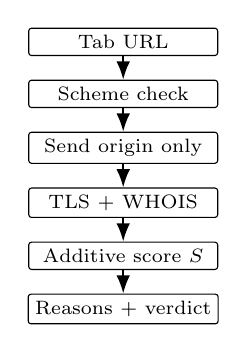
\begin{tikzpicture}[
  font=\scriptsize,
  sbox/.style={draw, rounded corners=1pt, align=center, inner sep=2.5pt, minimum width=2.4cm},
  arr/.style={-{Latex}, thick}
]
\node[sbox] (a) {Tab URL};
\node[sbox, below=3mm of a] (b) {Scheme check};
\node[sbox, below=3mm of b] (c) {Send origin only};
\node[sbox, below=3mm of c] (d) {TLS + WHOIS};
\node[sbox, below=3mm of d] (e) {Additive score $S$};
\node[sbox, below=3mm of e] (f) {Reasons + verdict};
\draw[arr] (a) -- (b);
\draw[arr] (b) -- (c);
\draw[arr] (c) -- (d);
\draw[arr] (d) -- (e);
\draw[arr] (e) -- (f);
\end{tikzpicture}
\caption{Implemented website scanning workflow in the WebSentinel prototype.}
\label{fig:flow}
\end{figure}

\subsection{Scoring Pipeline}
Fig.~\ref{fig:risk} shows how indicators enter $S$. Machine-learning fusion via~\eqref{eq:raw}--\eqref{eq:norm} is drawn as a planned input.

\begin{figure}[!t]
\centering
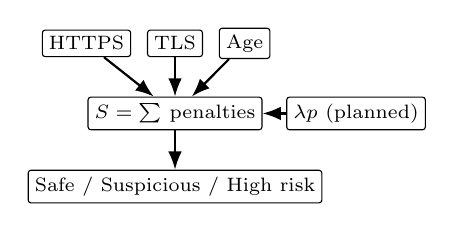
\begin{tikzpicture}[
  font=\scriptsize,
  n/.style={draw, align=center, inner sep=2.4pt, rounded corners=1pt},
  arr/.style={-{Latex}, thick}
]
\node[n] (h) {HTTPS};
\node[n, right=2mm of h] (t) {TLS};
\node[n, right=2mm of t] (g) {Age};
\node[n, below=5mm of t] (s) {$S=\sum$ penalties};
\node[n, below=5mm of s] (v) {Safe / Suspicious / High risk};
\node[n, right=3mm of s] (p) {$\lambda p$ (planned)};
\draw[arr] (h) -- (s);
\draw[arr] (t) -- (s);
\draw[arr] (g) -- (s);
\draw[arr] (p) -- (s);
\draw[arr] (s) -- (v);
\end{tikzpicture}
\caption{Risk-score pipeline. Prototype bands are $S<24$, $S<59$, and $S\ge 59$.}
\label{fig:risk}
\end{figure}

\subsection{Planned ML Pipeline}
Fig.~\ref{fig:ml} records the intended learning workflow. It is a design, not an executed experiment.

\begin{figure}[!t]
\centering
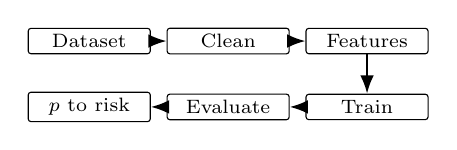
\begin{tikzpicture}[
  font=\scriptsize,
  n/.style={draw, align=center, inner sep=2.2pt, rounded corners=1pt, minimum width=1.55cm},
  arr/.style={-{Latex}, thick}
]
\node[n] (d) {Dataset};
\node[n, right=2mm of d] (c) {Clean};
\node[n, right=2mm of c] (f) {Features};
\node[n, below=5mm of f] (m) {Train};
\node[n, left=2mm of m] (e) {Evaluate};
\node[n, left=2mm of e] (p) {$p$ to risk};
\draw[arr] (d) -- (c);
\draw[arr] (c) -- (f);
\draw[arr] (f) -- (m);
\draw[arr] (m) -- (e);
\draw[arr] (e) -- (p);
\end{tikzpicture}
\caption{Planned machine-learning pipeline. No trained weights exist in the inspected repository.}
\label{fig:ml}
\end{figure}

\section{Experimental Setup}
\label{sec:setup}
This section specifies how evaluation \emph{should} be conducted. Measured hardware, dataset cardinalities, and metrics were not found (no notebooks, CSV metric dumps, or scan logs accompanied a completed study). Placeholders mark every missing quantity.

\subsection{Hardware and Software Environment}
\begin{itemize}
  \item Hardware: [INSERT HARDWARE CONFIGURATION]
  \item Operating system: [INSERT OS]
  \item Prototype runtime: Node.js with Express~5, axios, cheerio, and ssl-checker, as declared in \texttt{backend/package.json}
  \item Proposed runtime: Python, FastAPI, PostgreSQL, Redis, React/TypeScript
  \item Browser for the popup: Chromium-based, Manifest V3
\end{itemize}

\subsection{Datasets}
A future ML evaluation should name a licensed source, for example the Hannousse--Yahiouche web-page phishing set (11\,430 URLs, 87 features, balanced classes)~\cite{hannousse2021dataset} or a freshly sampled PhishTank/OpenPhish plus a documented legitimate crawl. Required fields:
\begin{itemize}
  \item Dataset name and license: [INSERT DATASET]
  \item Total URLs: [INSERT DATASET SIZE]
  \item Legitimate count: [INSERT LEGITIMATE URL COUNT]
  \item Phishing count: [INSERT PHISHING URL COUNT]
  \item Collection dates: [INSERT COLLECTION WINDOW]
  \item Train/test split: [INSERT TRAIN/TEST SPLIT]
\end{itemize}
The prototype rule engine can be evaluated without a trained model by scoring a labeled hold-out and reporting precision and recall of the three-level verdict after a documented mapping from labels to verdicts. That experiment has not been executed in the inspected materials.

\subsection{Metrics}
Classification: accuracy, precision, recall, F1-score, ROC-AUC, and confusion-matrix counts, with explicit false-negative analysis. System: wall-clock scan latency, timeout rate, and collector error rate. Security: SSRF test-case pass rate. Usability (optional, planned): whether non-experts understand the reason list.

\subsection{Security Test Methodology}
Security testing should combine (i)~unit tests for URL and address-policy functions, (ii)~negative tests that attempt loopback, RFC~1918, link-local, and metadata targets, (iii)~redirect-rebinding cases, and (iv)~an OWASP ZAP baseline against the WebSentinel application itself---not against third-party scanned sites~\cite{owaspzap,owasp2021top10}. Authorization to scan is limited to public information and the team's own deployment.

\section{Testing and Evaluation}
\label{sec:eval}
A complete program would include unit, integration, API, frontend, end-to-end, security, performance, and ML evaluation layers. The inspected \texttt{package.json} defines a single assertion: \texttt{parseCheckTarget('chrome://extensions')} must be marked unsupported. No pytest, Vitest, Playwright, or ZAP configuration was present. The following suite is therefore a plan, and Table~\ref{tab:functional} remains unfilled.

\subsection{Unit Testing}
Functions under test include scheme parsing, origin extraction, age-bucket selection, WHOIS date parsing, and (once written) address-policy predicates. The planned tool is pytest for Python and the existing Node test entry until the backend migrates.

\subsection{Integration and API Testing}
\texttt{POST /check} should be exercised with valid HTTPS hosts, HTTP hosts, malformed JSON, oversized bodies, and unsupported schemes. Expected statuses are 200 for completed checks, 400 for validation failures, and 500 only for unexpected collector collapse. \texttt{GET /health} should remain cheap and side-effect free.

\subsection{Frontend and End-to-End Testing}
Vitest can cover origin stripping and verdict mapping. Playwright should drive the popup (or future React app) through happy path, unsupported scheme, timeout, and API-error states.

\subsection{Security Testing}
OWASP ZAP~\cite{owaspzap} should scan the WebSentinel origin for common web flaws. Separate white-box tests must verify that private destinations never produce an outbound fetch. Until those tests exist, the prototype must not be described as SSRF-safe.

\subsection{Performance Testing}
Record elapsed time of \texttt{/check} under the five website classes in Table~\ref{tab:scan-perf}. Collector timeouts of 8~s bound worst-case latency in the prototype; measured averages are [RESULT REQUIRED].

\subsection{Machine-Learning Evaluation}
Once a model exists, report Table~\ref{tab:ml-results} with cross-validation or a chronological split to reduce leakage from near-duplicate campaigns~\cite{xiang2011cantinaplus,hannousse2021benchmark}. Analyze false negatives individually: a missed banking clone is more severe than a missed generic spam page.

\subsection{Functional Test Matrix}
Table~\ref{tab:functional} lists scenarios that follow from the methodology. Observed cells must stay marked until execution.

\begin{table*}[!t]
\centering
\caption{Planned functional test matrix. Observed cells are not filled because no executed suite was found.}
\label{tab:functional}
\renewcommand{\arraystretch}{1.08}
\begin{tabular}{>{\raggedright\arraybackslash}p{3.5cm}>{\raggedright\arraybackslash}p{4.4cm}>{\raggedright\arraybackslash}p{3.4cm}l}
\toprule
Scenario & Expected result & Observed & Status \\
\midrule
Valid HTTPS website & Score and reason list & [RESULT REQUIRED] & [RESULT REQUIRED] \\
HTTP website & $+20$ HTTPS penalty & [RESULT REQUIRED] & [RESULT REQUIRED] \\
Invalid / unsupported URL & Local or HTTP 400 reject & [RESULT REQUIRED] & [RESULT REQUIRED] \\
Expired or invalid TLS & Certificate warning & [RESULT REQUIRED] & [RESULT REQUIRED] \\
Long redirect chain & Planned warning & [RESULT REQUIRED] & [RESULT REQUIRED] \\
Recently registered domain & Age penalty & [RESULT REQUIRED] & [RESULT REQUIRED] \\
Suspicious lexical URL & Planned warning & [RESULT REQUIRED] & [RESULT REQUIRED] \\
Known phishing URL & Elevated caution & [RESULT REQUIRED] & [RESULT REQUIRED] \\
DNS failure & Degraded, no crash & [RESULT REQUIRED] & [RESULT REQUIRED] \\
Collector timeout & User-visible timeout & [RESULT REQUIRED] & [RESULT REQUIRED] \\
Private / loopback / metadata URL & Planned SSRF block & [RESULT REQUIRED] & [RESULT REQUIRED] \\
Oversized response & Planned abort & [RESULT REQUIRED] & [RESULT REQUIRED] \\
\bottomrule
\end{tabular}
\end{table*}

\section{Results and Discussion}
\label{sec:results}
No experimental campaign, labeled-score spreadsheet, or ML metric file was available. This section therefore reports only qualitative observations that follow directly from source inspection, and it leaves quantitative tables as templates.

\subsection{What Can Be Stated Without Fabrication}
The prototype returns a numeric $S$, a three-level message, and zero or more reason strings. Domain youth is the heaviest implemented penalty ($+35$), which is consistent with literature that treats registration age as a strong external feature~\cite{ma2009beyond,hannousse2021benchmark}. Invalid TLS and missing HTTPS are each $+20$, so an HTTP site with a failed certificate check can already reach the ``Suspicious'' band without being young. DNSSEC can reduce $S$ by 3, a small bonus that cannot cancel a new-domain penalty. The theoretical maximum under mutually exclusive age buckets is $20+20+35+10=85$ (HTTP, invalid TLS, age $<7$ days, WHOIS update $<7$ days), so the displayed denominator 100 is a scale, not a reachable sum of the current rule set.

\subsection{Missing Quantitative Results}
Tables~\ref{tab:ml-results}--\ref{tab:scan-perf} must be populated from measurements. Until then, claims of detection rate, latency, or test-pass percentage are unwarranted.

\begin{table}[!t]
\centering
\caption{Phishing classification performance. Values require a trained and evaluated model.}
\label{tab:ml-results}
\begin{tabular}{lccccc}
\toprule
Model & Acc. & Prec. & Rec. & F1 & AUC \\
\midrule
Logistic regression & --- & --- & --- & --- & --- \\
Decision tree & --- & --- & --- & --- & --- \\
Random forest & --- & --- & --- & --- & --- \\
Gradient boosting & --- & --- & --- & --- & --- \\
\bottomrule
\end{tabular}
\vspace{1pt}
{\footnotesize Each ``---'' stands for [RESULT REQUIRED]. Do not replace with invented numbers.}
\end{table}

\begin{table}[!t]
\centering
\caption{Security-module test results after the planned suite is executed.}
\label{tab:module-tests}
\begin{tabular}{lcccc}
\toprule
Module & Cases & Pass & Fail & Rate \\
\midrule
URL validation & --- & --- & --- & --- \\
Protocol / TLS & --- & --- & --- & --- \\
Domain / WHOIS & --- & --- & --- & --- \\
Risk scoring & --- & --- & --- & --- \\
SSRF policy & --- & --- & --- & --- \\
\bottomrule
\end{tabular}
\end{table}

\begin{table}[!t]
\centering
\caption{Scan performance of \texttt{POST /check} or the future scan API.}
\label{tab:scan-perf}
\begin{tabular}{lccc}
\toprule
Website type & Mean & Min & Max \\
\midrule
Established HTTPS & --- & --- & --- \\
HTTP-only & --- & --- & --- \\
Newly registered & --- & --- & --- \\
Invalid TLS & --- & --- & --- \\
Timeout / DNS failure & --- & --- & --- \\
\bottomrule
\end{tabular}
\end{table}

\subsection{Discussion}
The implemented reason list is the prototype's main user-facing contribution: it operationalizes the finding that users need more than a padlock~\cite{dhamija2006why}. The same list, however, can over-warn on legitimate new businesses and under-warn on aged, certificated clones---a known limitation of host-feature systems~\cite{xiang2011cantinaplus,lin2021phishpedia}. Adding lexical, redirect, and visual-brand signals is therefore well motivated, provided each new signal remains explainable and ethically collected. Dependence on a scraped WHOIS page is a reliability risk; RDAP would be the standards-compliant replacement~\cite{rfc7480}.

\section{Security and Privacy Considerations}
\label{sec:privacy}

\subsection{Safe Scanning}
Collectors must behave as unauthenticated public clients. The design forbids exploit payloads, credential posting, and authenticated crawling.

\subsection{SSRF and Abuse}
Section~\ref{sec:ssrf} is the primary technical control discussion. Rate limiting, authentication of the API, and refusing to become an open relay are required before wide deployment. The prototype's open CORS policy (\texttt{origin: true}) is convenient for a demo and overly permissive for production.

\subsection{Privacy and Storage Minimization}
The extension's privacy policy (29~August~2026) states that only the origin is transmitted, that path and query remain on device, and that names, passwords, payment details, accounts, and cross-tab history are not collected. That policy matches \texttt{frontend/app.js}. Planned databases should store the assessed origin, collector outputs, and reasons---not page cookies or form bodies. Retention limits are [INSERT RETENTION POLICY].

\subsection{API-Key and Third-Party Security}
Future reputation or breach APIs must keep keys in server-side secrets, never in the extension. The current WHOIS HTML provider is an implicit third party and should be replaced or contractually documented.

\subsection{Input Validation}
JSON body size is already capped at 8~kB. Further validation should constrain hostname length and character set after IDN decoding.

\subsection{Ethical Considerations}
Advisory language in the UI already declines to guarantee safety. Published papers and demonstrations should use owned or publicly documented URLs and licensed phishing datasets, not live credential-harvesting sites for interactive login tests.

\section{Limitations}
\label{sec:limit}
The following limitations are inherent or presently observed.
\begin{itemize}
  \item Dependence on third-party WHOIS presentation HTML, and, later, on threat-intelligence quotas.
  \item Incomplete RDAP coverage and redacted registration fields.
  \item False positives on new legitimate domains; false negatives on aged, well-certificated phishing.
  \item Rapid campaign turnover and dataset drift~\cite{hannousse2021benchmark,apwg2024q4}.
  \item No JavaScript execution or DOM analysis in the prototype; CAPTCHAs and heavily client-rendered pages will defeat naive HTML fetches.
  \item CDN and anycast hosting obscure geolocation even when IP lookup is added.
  \item HTTPS does not imply legitimacy.
  \item No trained ML model, hence no measured generalization and no SHAP study.
  \item Adversaries can manipulate lexical features and obtain free certificates.
  \item Network latency and external-API timeouts degrade completeness.
  \item Prototype SSRF policy is incomplete for resolved private addresses.
  \item No scan history, authentication, monitoring, or report pipeline in the inspected code.
\end{itemize}

\section{Future Work}
\label{sec:future}
Planned work, none of which is claimed as implemented, includes: replacing WHOIS scraping with RDAP; DNS, redirect, technology, and IP/hosting collectors; approved reputation and breach APIs; a documented ML ensemble or gradient-boosted model~\cite{dasguptta2024hybrid,hannousse2021benchmark}; SHAP explanations~\cite{lundberg2017shap}; PostgreSQL-backed history; downloadable reports; authenticated users; monitoring with change alerts; stronger brand-impersonation checks, including visual or logo methods in the spirit of Phishpedia and VisualPhishNet~\cite{lin2021phishpedia,abdelnabi2020visualphishnet}; DOM and login-form analysis; NLP on URL tokens~\cite{sahingoz2019ml}; graph-based domain infrastructure features; a production SSRF resolver guard; email-gateway integration; and cloud deployment with HTTPS, logs, and backups. Deep learning on raw URLs~\cite{aljofey2020cnn} is a candidate only after a simpler tabular baseline is measured.

\section{Conclusion}
\label{sec:concl}
Users cannot reasonably assemble protocol, certificate, and registration evidence every time they receive a link, and HTTPS does not resolve that problem. This paper presented WebSentinel as an explainable website security assessment: a proposed multi-collector architecture with a weighted risk model, a planned learning and SHAP pipeline, and a scanner threat model that treats SSRF as a core design constraint. Inspection of the current implementation shows a narrower but real system---a browser extension and Express service that score HTTPS, TLS, and domain age and that already explain each fired rule---rather than the full FastAPI, PostgreSQL, and machine-learning platform described for later capstone phases. No classification accuracies or latency statistics were invented. The practical usefulness of the present prototype is therefore limited to advisory, origin-scoped checks; the research value of the paper is the precise specification of how those checks should grow, how they should be measured, and how they must remain ethically passive. Completing the evaluation tables, closing the SSRF gaps, and training a documented model on a licensed dataset are the necessary next steps before any claim of detection performance can be made.

\section*{Acknowledgment}
The authors thank the remaining project members for implementation and testing support. Institutional names and funding statements should be inserted here before conference submission: [INSERT ACKNOWLEDGMENT].

\begin{thebibliography}{00}

\bibitem{dhamija2006why}
R.~Dhamija, J.~D. Tygar, and M.~Hearst, ``Why phishing works,'' in \emph{Proc. SIGCHI Conf. Human Factors Comput. Syst. (CHI)}, 2006, pp. 581--590.

\bibitem{zhang2007cantina}
Y.~Zhang, J.~I. Hong, and L.~F. Cranor, ``{CANTINA}: A content-based approach to detecting phishing web sites,'' in \emph{Proc. 16th Int. Conf. World Wide Web (WWW)}, 2007, pp. 639--648.

\bibitem{ma2009beyond}
J.~Ma, L.~K. Saul, S.~Savage, and G.~M. Voelker, ``Beyond blacklists: Learning to detect malicious web sites from suspicious {URLs},'' in \emph{Proc. 15th ACM SIGKDD Int. Conf. Knowl. Discovery Data Mining (KDD)}, 2009, pp. 1245--1254.

\bibitem{ma2009identifying}
J.~Ma, L.~K. Saul, S.~Savage, and G.~M. Voelker, ``Identifying suspicious {URLs}: An application of large-scale online learning,'' in \emph{Proc. 26th Int. Conf. Mach. Learn. (ICML)}, 2009, pp. 681--688.

\bibitem{whittaker2010large}
C.~Whittaker, B.~Ryner, and M.~Nazif, ``Large-scale automatic classification of phishing pages,'' in \emph{Proc. Netw. Distrib. Syst. Security Symp. (NDSS)}, 2010.

\bibitem{xiang2011cantinaplus}
G.~Xiang, J.~Hong, C.~P. Rose, and L.~Cranor, ``{CANTINA+}: A feature-rich machine learning framework for detecting phishing web sites,'' \emph{ACM Trans. Inf. Syst. Secur.}, vol.~14, no.~2, pp. 21:1--21:28, 2011.

\bibitem{marchal2014phishstorm}
S.~Marchal, J.~Fran\c{c}ois, R.~State, and T.~Engel, ``{PhishStorm}: Detecting phishing with streaming analytics,'' \emph{IEEE Trans. Netw. Service Manag.}, vol.~11, no.~4, pp. 458--471, Dec. 2014.

\bibitem{mohammad2014predicting}
R.~M. Mohammad, F.~Thabtah, and L.~McCluskey, ``Predicting phishing websites based on self-structuring neural network,'' \emph{Neural Comput. Appl.}, vol.~25, no.~2, pp. 443--458, 2014.

\bibitem{ribeiro2016lime}
M.~T. Ribeiro, S.~Singh, and C.~Guestrin, ```Why should {I} trust you?': Explaining the predictions of any classifier,'' in \emph{Proc. 22nd ACM SIGKDD Int. Conf. Knowl. Discovery Data Mining (KDD)}, 2016, pp. 1135--1144.

\bibitem{lundberg2017shap}
S.~M. Lundberg and S.-I. Lee, ``A unified approach to interpreting model predictions,'' in \emph{Proc. Adv. Neural Inf. Process. Syst. (NeurIPS)}, 2017, pp. 4765--4774.

\bibitem{niakanlahiji2018phishmon}
A.~Niakanlahiji, B.-T. Chu, and E.~Al-Shaer, ``{PhishMon}: A machine learning framework for detecting phishing webpages,'' in \emph{Proc. IEEE Int. Conf. Intell. Security Informat. (ISI)}, 2018, pp. 220--225.

\bibitem{rao2019detection}
R.~S. Rao and A.~R. Pais, ``Detection of phishing websites using an efficient feature-based machine learning framework,'' \emph{Neural Comput. Appl.}, vol.~31, no.~8, pp. 3851--3873, 2019.

\bibitem{sahingoz2019ml}
O.~K. Sahingoz, E.~Buber, O.~Demir, and B.~Diri, ``Machine learning based phishing detection from {URLs},'' \emph{Expert Syst. Appl.}, vol.~117, pp. 345--357, Mar. 2019.

\bibitem{rao2019catchphish}
R.~S. Rao, T.~Vaishnavi, and A.~R. Pais, ``{CatchPhish}: Detection of phishing websites by inspecting {URLs},'' \emph{J. Ambient Intell. Humaniz. Comput.}, vol.~11, pp. 813--825, 2020.

\bibitem{aljofey2020cnn}
A.~Aljofey, Q.~Jiang, Q.~Qu, M.~Huang, and J.-P. Niyigena, ``An effective phishing detection model based on character level convolutional neural network from {URL},'' \emph{Electronics}, vol.~9, no.~9, p.~1514, 2020.

\bibitem{abdelnabi2020visualphishnet}
S.~Abdelnabi, K.~Krombholz, and M.~Fritz, ``{VisualPhishNet}: Zero-day phishing website detection by visual similarity,'' in \emph{Proc. ACM SIGSAC Conf. Comput. Commun. Security (CCS)}, 2020, pp. 1681--1698.

\bibitem{lin2021phishpedia}
Y.~Lin \emph{et al.}, ``{Phishpedia}: A hybrid deep learning based approach to visually identify phishing webpages,'' in \emph{Proc. 30th {USENIX} Security Symp.}, 2021, pp. 3793--3810.

\bibitem{hannousse2021benchmark}
A.~Hannousse and S.~Yahiouche, ``Towards benchmark datasets for machine learning based website phishing detection: An experimental study,'' \emph{Eng. Appl. Artif. Intell.}, vol.~104, p.~104347, 2021.

\bibitem{dasguptta2024hybrid}
S.~Das Guptta, K.~T. Shahriar, H.~Alqahtani, D.~Alsalman, and I.~H. Sarker, ``Modeling hybrid feature-based phishing websites detection using machine learning techniques,'' \emph{Ann. Data Sci.}, vol.~11, no.~1, pp. 217--242, 2024.

\bibitem{rfc3986}
T.~Berners-Lee, R.~Fielding, and L.~Masinter, ``Uniform resource identifier ({URI}): Generic syntax,'' IETF RFC~3986, 2005.

\bibitem{rfc1035}
P.~Mockapetris, ``Domain names---implementation and specification,'' IETF RFC~1035, 1987.

\bibitem{rfc1918}
Y.~Rekhter, B.~Moskowitz, D.~Karrenberg, G.~J. de Groot, and E.~Lear, ``Address allocation for private Internets,'' IETF RFC~1918, 1996.

\bibitem{rfc5280}
D.~Cooper \emph{et al.}, ``Internet {X.509} public key infrastructure certificate and certificate revocation list ({CRL}) profile,'' IETF RFC~5280, 2008.

\bibitem{rfc6890}
M.~Cotton, L.~Vegoda, R.~Bonica, and B.~Haberman, ``Special-purpose {IP} address registries,'' IETF RFC~6890, 2013.

\bibitem{rfc7480}
A.~Newton, B.~Ellacott, and N.~Kong, ``{HTTP} usage in the registration data access protocol ({RDAP}),'' IETF RFC~7480, 2015.

\bibitem{rfc7483}
S.~Hollenbeck and A.~Newton, ``{JSON} responses for the registration data access protocol ({RDAP}),'' IETF RFC~7483, 2015.

\bibitem{rfc8446}
E.~Rescorla, ``The transport layer security ({TLS}) protocol version 1.3,'' IETF RFC~8446, 2018.

\bibitem{rfc9110}
R.~Fielding, M.~Nottingham, and J.~Reschke, ``{HTTP} semantics,'' IETF RFC~9110, 2022.

\bibitem{owasp2021top10}
{OWASP Foundation}, ``{OWASP} Top 10:2021,'' 2021. [Online]. Available: \url{https://owasp.org/Top10/}

\bibitem{owaspssrf}
{OWASP Foundation}, ``Server-side request forgery prevention cheat sheet.'' [Online]. Available: \url{https://cheatsheetseries.owasp.org/cheatsheets/Server_Side_Request_Forgery_Prevention_Cheat_Sheet.html}

\bibitem{apwg2024q4}
{Anti-Phishing Working Group}, ``Phishing activity trends report, 4th quarter 2024,'' Mar. 2025. [Online]. Available: \url{https://apwg.org/trendsreports/}

\bibitem{hannousse2021dataset}
A.~Hannousse and S.~Yahiouche, ``Web page phishing detection,'' Mendeley Data, V3, 2021, doi: 10.17632/c2gw7fy2j4.3.

\bibitem{owaspzap}
{OWASP Foundation}, ``{OWASP ZED} attack proxy ({ZAP}).'' [Online]. Available: \url{https://www.zaproxy.org/}

\end{thebibliography}

\end{document}
